\problemname{Eszett}
\illustration{0.31}{prompt}{A demonstration of the \texttt{upper} function in Python\vspace{-0.5cm}}%
For those trying to learn German, the letter `ß', called \emph{Eszett} or \emph{sharp S},
is usually a source of great confusion.
This letter is unique to the German language and it looks similar to a `b' but is pronounced like an `s'.

Adding to the confusion is the fact that, until a few years ago, only a lowercase version of `ß' existed in standard German orthography.
Wherever an uppercase `ß' was needed, for example in legal documents and shop signs,
it was (and usually still is) replaced by capital double letters `SS'.
In 2017, the capital `\scalerel*{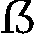
\includegraphics{eszett}}{B}' was officially introduced into
the German language and may now be used in those scenarios, instead.

Other than being confusing for foreigners, the practice of replacing `ß' with
`SS' also introduces some ambiguity because a given uppercase word
featuring one or more occurrences of `SS' may correspond to multiple different
lowercase words, depending on whether each `SS' is a capitalized `ß` or `ss'.

Given one uppercase word, find all the lowercase words
that it could be derived from.
As the letter `ß' is not part of the ASCII range,
please write an uppercase `B', instead.

\begin{Input}
  The input consists of:
  \begin{itemize}
    \item One line with a string $s$ ($1 \le |s| \le 20$) consisting of uppercase letters.
  \end{itemize}
  It is guaranteed that the letter \texttt{S} occurs at most three times in $s$.
  Note that $s$ need not be an actual German word.
\end{Input}

\begin{Output}
  Output all the possible lowercase strings corresponding to $s$. Any order
  will be accepted, but each string must occur exactly once.
\end{Output}
